\usetikzlibrary{positioning,arrows}
\tikzset{%
  >=latex, % option for nice arrows
  inner sep=0pt,%
  outer sep=2pt,%
  mark coordinate/.style={inner sep=0pt,outer sep=0pt,minimum size=3pt,
    fill=black,circle}%
}
\tikzstyle{roundnode}=[circle, draw=green!60, fill=green!5, very thick, minimum size=7mm]
\tikzstyle{squarenode}=[rectangle, draw=red!60, fill=red!5, very thick, minimum size=5mm]
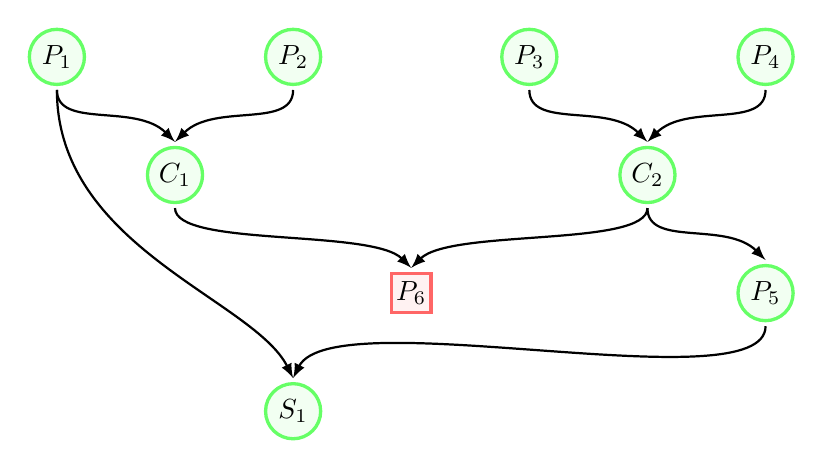
\begin{tikzpicture}
  \begin{scope}[yshift=8cm,node distance=1.5cm and 1.5cm]
%Nodes
\node[roundnode]      (p1)                                {$P_1$};
\node               (dummy1)          [right of=p1]             {};
\node[roundnode]        (p2)       [right of=dummy1]             {$P_2$};
\node                 (dummy2)      [right of=p2]             {};
\node[roundnode]         (p3)       [right of=dummy2]             {$P_3$};
\node                 (dummy3)      [right of=p3]               {};
\node[roundnode]        (p4)       [right of=dummy3]            {$P_4$};
\node[roundnode]       (c1)       [below of =dummy1]            {$C_1$};
\node                 (dummy4)       [right of= c1] {};
\node                 (dummy5)       [right of= dummy4] {};
\node[roundnode]       (c2)       [below of=dummy3]            {$C_2$};
\node[squarenode]        (p6)       [below of=dummy5]            {$P_6$};
\node                 (dummy6)       [right of= c2] {};
\node[roundnode]        (p5)       [below of=dummy6]            {$P_5$};
\node                 (dummy7)       [left of= p6] {};
\node[roundnode]        (s1)       [below of=dummy7]            {$S_1$};
%Lines
\draw[-latex, thick] (p1.south) .. controls +(0cm,-0.5cm) and +(-0.5cm,0.5cm) ..  (c1.north);
\draw[-latex, thick] (p2.south) .. controls +(0cm,-0.5cm) and +(0.5cm,0.5cm) .. (c1.north);
\draw[-latex,thick] (p3.south) .. controls +(0cm,-0.5cm) and +(-0.5cm,0.5cm) .. (c2.north);
\draw[-latex, thick] (p4.south) .. controls +(0cm,-0.5cm) and +(0.5cm,0.5cm) .. (c2.north);
\draw[-latex,thick] (c1.south) .. controls +(0cm,-0.5cm) and +(-0.5cm,0.5cm) .. (p6.north);
\draw[-latex, thick] (c2.south) .. controls +(0cm,-0.5cm) and +(0.5cm,0.5cm) .. (p6.north);
\draw[-latex,thick] (c2.south) .. controls +(0cm,-0.5cm) and +(-0.5cm,0.5cm) .. (p5.north);
\draw[-latex,thick] (p1.south) .. controls +(0cm,-2cm) and +(-0.5cm,1cm) .. (s1.north);
\draw[-latex, thick] (p5.south) .. controls +(0cm,-1cm) and +(0.5cm,1cm) .. (s1.north);
  \end{scope}
%\draw[->] (rightsquare.south) .. controls +(down:7mm) and +(right:7mm) .. (lowercircle.east);
\end{tikzpicture}